\documentclass[Main.tex]{subfiles}
\begin{document}
	\section{Bland-Altman Approach}

The issue of whether two measurement methods are comparable to the extent that they can be used interchangeably with sufficient accuracy is encountered frequently in scientific research. Historically comparison of two methods of measurement was carried
out by use of matched pairs correlation coefficients or simple bivariate methods. Bland and Altman recognized the inadequacies of these analyses and articulated quite thoroughly the basis on which of which they are unsuitable for comparing two methods of measurement \citep*{BA83}.
	


The scientific question at hand is the correct approach to
assessing whether two methods can be used interchangeably.
\citet{BA99} expresses this as follows:
\begin{quote}We want to
	know by how much (one) method is likely to differ from the
	(other), so that if it not enough to cause problems in the
	mathematical interpretation we can ... use the two
	interchangeably.
\end{quote}


Statisticians Martin Bland and Douglas Altman recognized the inadequacies of these analyzes and
articulated quite thoroughly the basis on which of which they are unsuitable for comparing two methods of measurement \citep*{BA83}. Furthermore they proposed their simple methodology specifically constructed for method comparison studies. They acknowledge the opportunity to apply other valid, but complex, methodologies, but argue that a simple approach is preferable, especially when the results must be `explained to non-statisticians'.

As an alternative they proposed a simple statistical methodology specifically appropriate for method comparison studies. They acknowledge that there are other valid methodologies, but argue that a simple approach is preferable to complex approaches,	\emph{"especially when the results must be explained to non-statisticians"} \citep*{BA83}.

	Bland-Altman plots are a powerful graphical methodology for making
	a visual assessment of the data. \citet*{BA83} express the
	motivation for this plot thusly:
	\begin{quote}
		``From this type of plot it is much easier to assess the magnitude
		of disagreement (both error and bias), spot outliers, and see
		whether there is any trend, for example an increase in
		(difference) for high values. This way of plotting the data is a
		very powerful way of displaying the results of a method comparison
		study."
	\end{quote}
	
	
\subsection{Identity Plot}
The first step recommended which the authors argue should be mandatory is construction of a simple scatter plot of the data.
The line of equality ($X=Y$) should also be shown, as it is	necessary to give the correct interpretation of how both methods
compare. 

Notwithstanding previous remarks about linear regression, the first step recommended, which the authors argue should be mandatory, is construction of a simple scatter plot of the data. The line of equality ($X=Y$) should also be shown, as it is necessary to give the correct interpretation of how both methods compare. In the case of good agreement, the observations would be distributed closely along the line of equality. A scatter plot of the Grubbs data is shown in Figure 1.1. A visual inspection thereof confirms the previous conclusion that there is an inter method bias present, i.e. Fotobalk device has a tendency to record a lower velocity.

\begin{figure}[h!]
	\begin{center}
		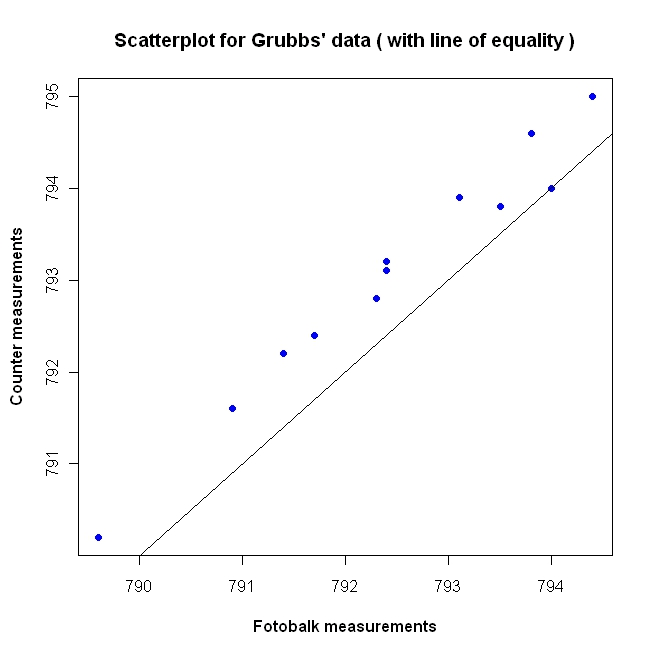
\includegraphics[width=130mm]{images/GrubbsScatter.jpeg}
		\caption{Scatter plot For Fotobalk and Counter Methods.}\label{GrubbsScatter}
	\end{center}
\end{figure}

The authors advise the use of scatter plots to identify outliers, and to determine if there is curvilinearity present. In the region of linearity, simple linear regression may yield results of interest.

\citet{Dewitte} notes that scatter plots were very seldom presented in the Annals of Clinical Biochemistry. This apparently results from the fact that the `Instructions for Authors' dissuade the use of regression analysis, which conventionally is accompanied by a scatter plot.



\subsection{Bland-Altman Plots}




In light of shortcomings associated with scatterplots, \citet*{BA83} recommend a further analysis of the data. Firstly
case-wise differences of measurements of two methods $d_{i} = y_{1i}-y_{2i} \mbox{ for }i=1,2,..n$ on the same subject should be calculated, and then the average of those measurements ($a_{i} = (y_{1i} + y_{2i})/2 \mbox{ for }i=1,2,..n$). These differences and
averages are then plotted. 

In 1986 Bland and Altman published a paper in the Lancet proposing the difference plot for use for method comparison purposes. It has
proved highly popular ever since. This is a simple, and widely used, plot of the differences of each data pair, and the corresponding average value. An important requirement is that the two measurement methods use the same scale of measurement.

Bland Altman have recommended the use of graphical techniques to assess agreement.
Principally their method is calculating, for each pair of corresponding two methods of measurement of some underlying quantity, with no replicate measurements, the difference and mean. Differences are then plotted against the mean.

The averages of the two measurements is considered by
	Bland and Altman to the best estimate for the unknown true value.
	Importantly both methods must measure with the same units. 
	
	These
	results are then plotted, with differences on the ordinate and
	averages on the abscissa (figure 1.2).



\citet{BA83} proposes a scatterplot of the case-wise averages and differences of two methods of measurement. This scatterplot has since become widely known as the Bland-Altman plot. \citet*{BA83} express the
motivation for this plot thusly:
\begin{quote}
	``From this type of plot it is much easier to assess the magnitude
	of disagreement (both error and bias), spot outliers, and see
	whether there is any trend, for example an increase in (difference) for high values. This way of plotting the data is a very powerful way of displaying the results of a method comparison study."
\end{quote}



The case wise-averages capture several aspects of the data, such as expressing the range over which the values were taken, and assessing whether the assumptions of constant variance holds.
Case-wise averages also allow the case-wise differences to be presented on a two-dimensional plot, with better data visualization qualities than a one dimensional plot. 

\citet{BA86} cautions that it would be the difference against either measurement value instead of their average, as the difference relates to both value. This approach has proved very popular, and the Bland-Altman plots is widely regarded as powerful graphical technique for making a visual assessment of the data.

The magnitude of the inter-method bias between the two methods is simply the average of the differences $\bar{d}$. This inter-method bias is represented with a line on the Bland-Altman plot. As the objective of the Bland-Altman plot is to advise on the agreement of two methods, it is the case-wise differences that are also particularly relevant. The variances around this bias is estimated by the standard deviation of these differences $S_{d}$. This inter-method bias is represented with a	line on the Bland-Altman plot. These estimates are only meaningful	if there is uniform inter-bias and variability throughout the range of measurements, which can be checked by visual inspection of the plot. 

\subsection{Using Bland-Altman Plots}
	
The Bland-Altman plot is simply a scatterplot of the case-wise
	averages and differences of two methods of measurement. As the
	objective of the Bland-Altman plot is to advise on the agreement
	of two methods, it is the case-wise differences that are particularly. Later it will be shown that case-wise differences are the sole component of the next part of the approach, the
	limits of agreement.
	
For creating plots, the case wise-averages fulfil several
	functions, such as expressing the range over which the values were
	taken, and assessing whether the assumptions of constant variance
	holds. 
	
Case-wise averages also allow the case-wise differences to be presented on a two-dimensional plot, with better data visualization qualities than a one dimensional plot. \citet{BA86} cautions that it would be the difference against either measurement value instead of their average, as the difference
	relates to both value.


\subsection{Bland-Altman plots for the Grubbs data}
These estimates are only meaningful if there is uniform inter-bias and variability throughout the
range of measurements, which can be checked by visual inspection of the plot. In the case of Grubbs data the inter-method bias is $-0.61$ metres per second, and is indicated by the dashed line on Figure 1.2. By inspection of the plot, it is also possible to
compare the precision of each method. Noticeably the differences tend to increase as the averages increase.


	
The Bland-Altman plot for comparing the `Fotobalk' and `Counter' methods, which shall henceforth be referred to as the `F vs C'
comparison,  is depicted in Figure 1.2, using data from Table 1.3. The presence and magnitude of the inter-method bias is indicated
	by the dashed line.

	


	
	\begin{table}[h!]
		\renewcommand\arraystretch{0.7}%
		\begin{center}
			\begin{tabular}{|c||c|c|c||c|c||c|c|}
				\hline

Round	&	Fotobalk	&	Counter	&	Terma	&		&		&		&		\\
&	F	&	C	&	T	&	F-C	&	F-T	&	[F+C/2]	&	F+T/2	\\ \hline
1	&	793.8	&	794.6	&	793.2	&	-0.8	&	0.6	&	794.2	&	793.5	\\
2	&	793.1	&	793.9	&	793.3	&	-0.8	&	-0.2	&	793.5	&	793.2	\\
3	&	792.4	&	793.2	&	792.6	&	-0.8	&	-0.2	&	792.8	&	792.5	\\
4	&	794	&	794	&	793.8	&	0	&	0.2	&	794	&	793.9	\\
5	&	791.4	&	792.2	&	791.6	&	-0.8	&	-0.2	&	791.8	&	791.5	\\
6	&	792.4	&	793.1	&	791.6	&	-0.7	&	0.8	&	792.75	&	792	\\
7	&	791.7	&	792.4	&	791.6	&	-0.7	&	0.1	&	792.05	&	791.65	\\
8	&	792.3	&	792.8	&	792.4	&	-0.5	&	-0.1	&	792.55	&	792.35	\\
9	&	789.6	&	790.2	&	788.5	&	-0.6	&	1.1	&	789.9	&	789.05	\\
10	&	794.4	&	795	&	794.7	&	-0.6	&	-0.3	&	794.7	&	794.55	\\
11	&	790.9	&	791.6	&	791.3	&	-0.7	&	-0.4	&	791.25	&	791.1	\\
12	&	793.5	&	793.8	&	793.5	&	-0.3	&	0	&	793.65	&	793.5	\\

				
				\hline
			\end{tabular}
			\caption{Fotobalk and Terma methods: differences and averages.}
		\end{center}
	\end{table}
	

	
	\begin{figure}[h!]
		\begin{center}
			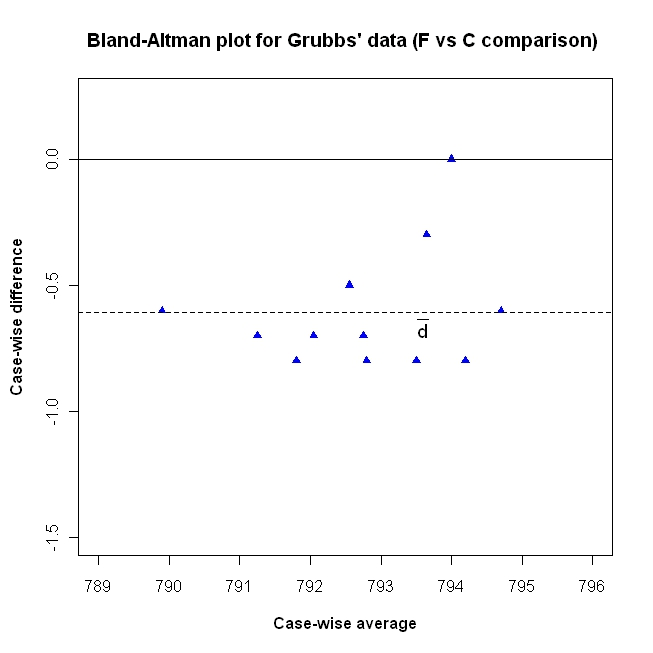
\includegraphics[width=120mm]{images/GrubbsBAplot-noLOA.jpeg}
			\caption{Bland-Altman plot For Fotobalk and Counter methods.}\label{GrubbsBA-noLOA}
		\end{center}
	\end{figure}
	
	
	
	In Figure 1.3 Bland-Altman plots for the `F vs C' and `F vs T'
	comparisons are shown, where `F vs T' refers to the comparison of
	the `Fotobalk' and `Terma' methods. Usage of the Bland-Altman plot
	can be demonstrate in the contrast between these comparisons. By inspection, there exists a larger inter-method bias in the `F vs C' comparison than in the `F vs T' comparison. Conversely there
	appears to be less precision in `F vs T' comparison, as indicated
	by the greater dispersion of covariates.
	
	\begin{figure}[h!]
		\begin{center}
			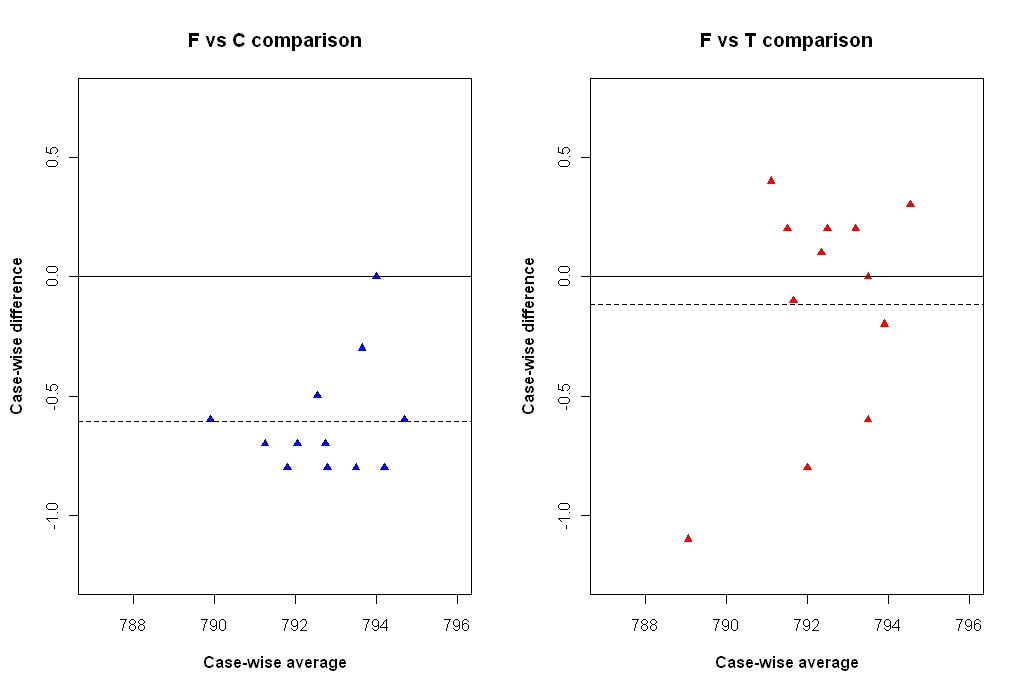
\includegraphics[height=90mm]{images/GrubbsDataTwoBAplots.jpeg}
			\caption{Bland-Altman plots for Grubbs' F vs C and F vs T comparisons.}\label{GrubbsDataTwoBAplots}
		\end{center}
	\end{figure}
	

	
	%	\begin{figure}[h!]
	%		\begin{center}
	%			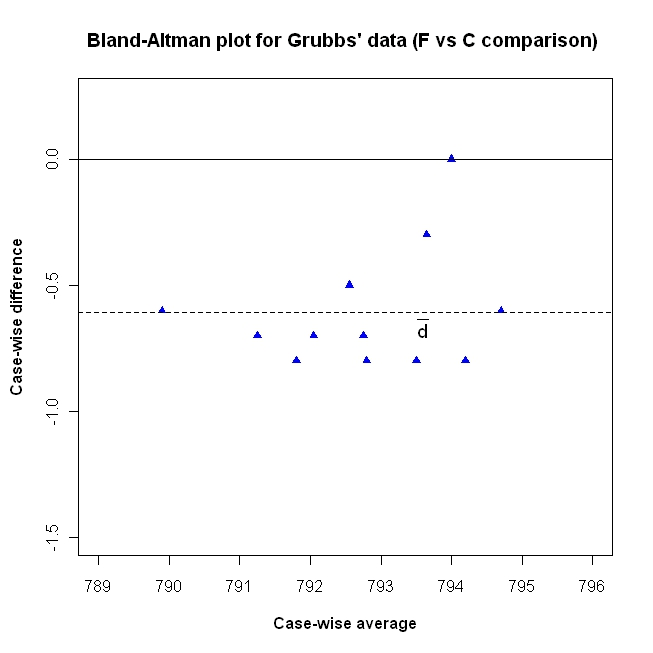
\includegraphics[width=120mm]{images/GrubbsBAplot-noLOA.jpeg}
	%			\caption{Bland-Altman plot For Fotobalk and Counter methods.}\label{GrubbsBA-noLOA}
	%		\end{center}
	%	\end{figure}
	%	
	%	

	
	%	\begin{figure}[h!]
	%		\begin{center}
	%			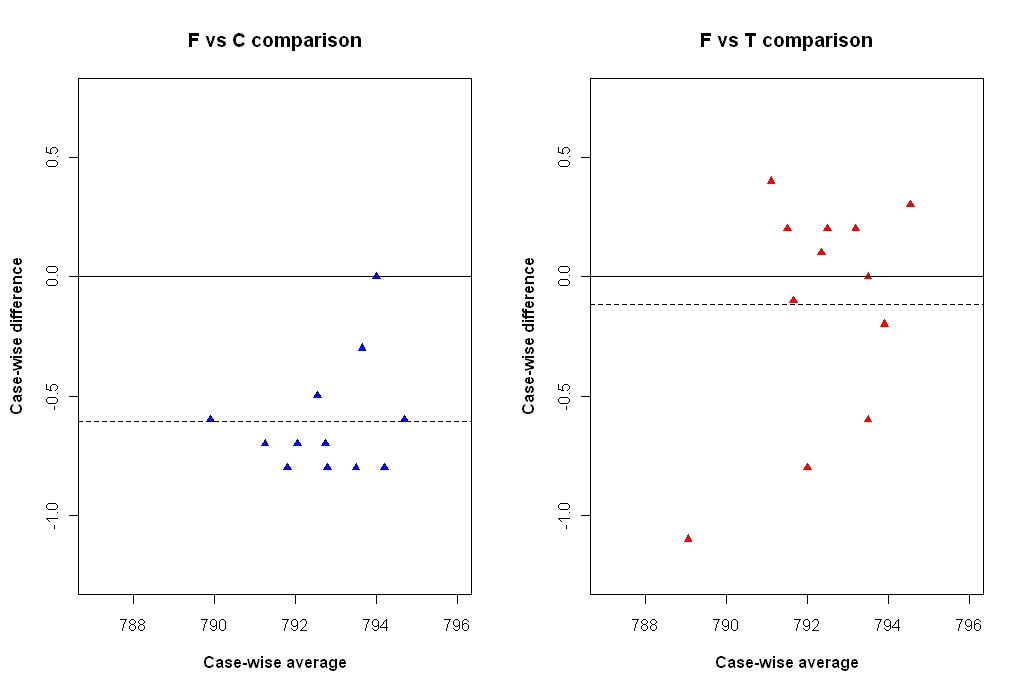
\includegraphics[height=90mm]{images/GrubbsDataTwoBAplots.jpeg}
	%			\caption{Bland-Altman plots for Grubbs' F vs C and F vs T comparisons.}\label{GrubbsDataTwoBAplots}
	%		\end{center}
	%	\end{figure}
	


\subsection{Bias Detection}
Further to this method, the presence of constant bias may be
indicated if the average value differences is not equal to zero. Bland and Altman does, however, indicate the indication of absence
of bias does not provide sufficient information to allow a judgement as to whether or not one method can be substituted for
another.


The dashed line in Figure 2.2 alludes to the inter method bias
	between the two methods, as mentioned previously. Bland and Altman
	recommend the estimation of inter method bias by calculating the
	average of the differences. In the case of Grubbs data the inter
	method bias is $-0.6083$ metres per second.

	\begin{figure}[h!]
		\begin{center}
			\includegraphics[width=120mm]{images/GrubbsBAplot.jpeg}
			\caption{Bland Altman Plot For Fotobalk and Counter Methods}\label{GrubbsBA}
		\end{center}
	\end{figure}

	By inspection of the plot, it is also possible to compare the precision of each method. Noticeably the differences tend to
	increase as the averages increase.
	
 	\subsection{Simulated Data}

Figures 1.3 1.4 and 1.5 are three Bland-Altman plots derived from
	simulated data, each for the purpose of demonstrating how the plot
	would inform an analyst of trends that would adversely affect use
	of the recommended approach. Figure 1.3 demonstrates how the
	Bland Altman plot would indicate increasing variance of
	differences over the measurement range. 
	
	
Figure 1.4, is an example of cases where the inter-method bias changes over the measurement range. This is known as proportional bias, and is defined by \citet{ludbrook97} as meaning that `one method gives values that are higher (or lower) than those from the other by an amount that is proportional to the level of the measured variable'.
	
	Figure 1.4 demonstrates how the Bland-Altman plot would indicate
	increasing variance of differences over the measurement range.
	Fitted regression lines, for both the upper and lower half of the
	plot, has been added to indicate the trend. 
	
Both of these cases violate the assumptions
	necessary for further analysis using limits of agreement ,which
	shall be discussed later. The plot also can be used to identify
	outliers. An outlier is an observation that is numerically distant
	from the rest of the data. Classification thereof is a subjective
	decision in any analysis, but must be informed by the logic of the
	formulation. Figure 1.5 is a Bland Altman plot with two
	conspicuous observations, at the extreme left and right of the
	plot respectively.
	
	
	%\begin{figure}[h!]
	%	\begin{center}
	%		\includegraphics[width=125mm]{BAOutliers.jpeg}
	%		\caption{Bland-Altman Plot indicating the presence of Outliers}\label{PropBias}
	%	\end{center}
	%\end{figure}
	
	In the Bland-Altman plot, the horizontal displacement of any
	observation is supported by two independent measurements. Hence
	any observation , such as the one on the extreme right of figure
	1.5, should not be considered an outlier on the basis of a
	noticeable horizontal displacement from the main cluster. The one
	on the extreme left should be considered an outlier, as it has a
	noticeable vertical displacement from the rest of the
	observations.
	
	\citet*{BA99} do not recommend excluding outliers from analyses.
	However recalculation of the inter-method bias estimate , and
	further calculations based upon that estimate, are useful for
	assessing the influence of outliers.\citep{BA99} states that
	\emph{"We usually find that this method of analysis is not too
		sensitive to one or two large outlying differences."}

	Application of regression techniques to the Bland-Altman 
	plot, and subsequent formal testing for the constant variability of differences is informative. The data set may be divided into two subsets, containing the observations wherein the difference values are less than and greater than the inter-method bias respectively.
	

	For both of these fits, hypothesis tests for the respective slopes
	can be performed. While both tests can be considered separately,
	multiple comparison procedures, such as the Benjamini-Hochberg
	\citep{BH} test, should be also be used.
	
	\begin{figure}[h!]
		\begin{center}
			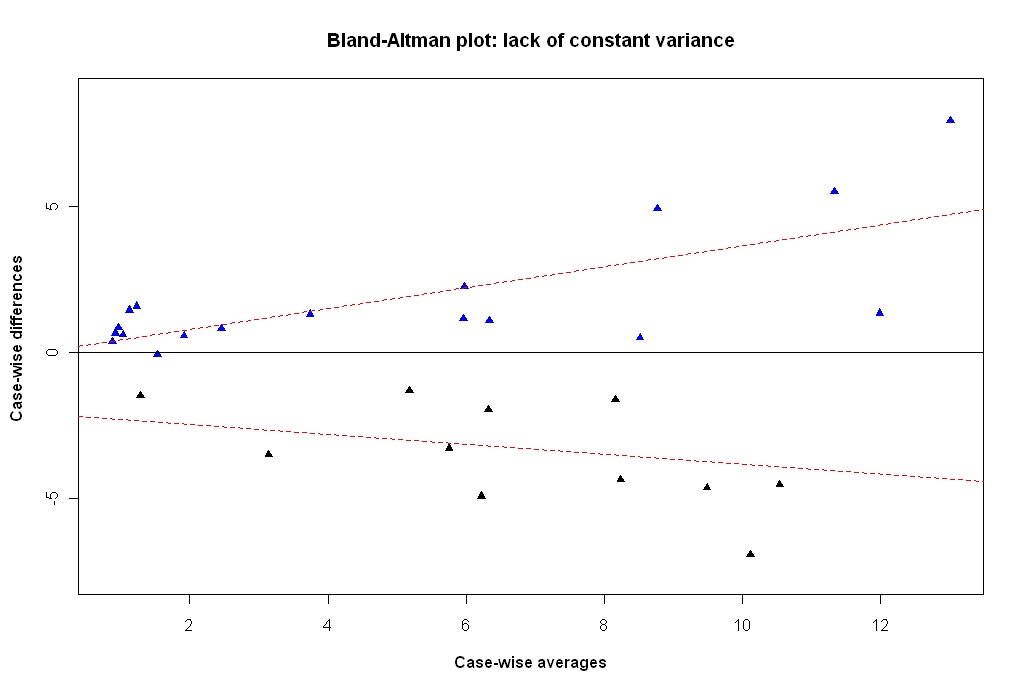
\includegraphics[height=90mm]{images/BAFanEffect.jpeg}
			\caption{Bland-Altman plot demonstrating the increase of variance over the range.}\label{BAFanEffect}
		\end{center}
	\end{figure}
	
	\begin{figure}[h!]
		\begin{center}
			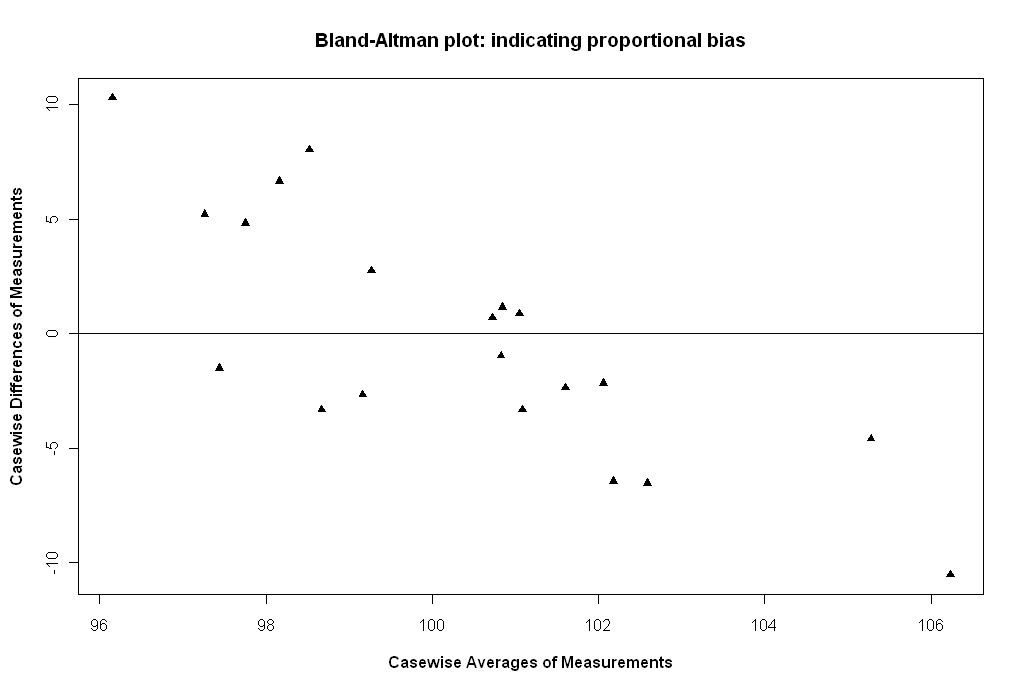
\includegraphics[height=90mm]{images/PropBias.jpeg}
			\caption{Bland-Altman plot indicating the presence of proportional bias.}\label{PropBias}
		\end{center}
	\end{figure}
	
	\begin{figure}[h!]
		\begin{center}
			\includegraphics[width=125mm]{images/BAOutliers.jpeg}
			\caption{Bland-Altman plot indicating the presence of potential outliers.}\label{Outliers}
		\end{center}
	\end{figure}


	\subsection{Adverse features}
	
	Estimates for inter-method bias and variance of differences are only meaningful if there is uniform inter-bias and variability throughout the range of measurements. Fulfilment of these assumptions can be checked by visual inspection of the plot. The prototype Bland-Altman plots depicted in Figures 1.4, 1.5 and 1.6 are derived from simulated data, for the purpose of demonstrating how the plot would inform an analyst of features that would adversely affect use of the recommended methodology.
	
	Figure 1.4 demonstrates how the Bland-Altman plot would indicate increasing variance of differences over the measurement range. Fitted regression lines, for both the upper and lower half of the plot, has been added to indicate the trend. 
	
 In both Figures 1.4 and 1.5, the assumptions necessary for further analysis using the limits of agreement are violated.
	




	

	\subsection{Variations of The Bland Altman Plot}

	Variations of the Bland Altman plot is the use of ratios, in the
	place of differences.
	\begin{equation}
	D_{i} = X_{i} - Y_{i}   \label{BA01}
	\end{equation}
	Altman and Bland suggest plotting the within subject differences $
	D = X_{1} - X_{2} $ on the ordinate versus the average of $x_{1}$
	and  $x_{2}$ on the abscissa.
	

	
\section{Conclusions about Existing Methodologies}

Scatterplots are recommended by \citet{BA83} for an initial
examination of the data, facilitating an initial judgement and helping to identify potential outliers. They are not useful for a thorough examination of the data. \citet{BritHypSoc} notes that data points will tend to cluster around the line of equality, obscuring interpretation.


The Bland Altman methodology is well noted for its ease of use, and can be easily implemented with most software packages. Also it
doesn't require the practitioner to have more than basic statistical training. The plot is quite informative about the variability of the differences over the range of measurements. For example, an inspection of the plot will indicate the 'fan effect'. They also can be used to detect the presence of an outlier.

\citet{ludbrook97,ludbrook02} criticizes these plots on the
basis that they presents no information on effect of constant bias
or proportional bias. These plots are only practicable when both methods measure in the same units. Hence they are totally
unsuitable for conversion problems. The limits of agreement are somewhat arbitrarily constructed. They may or may not be suitable
for the data in question. It has been found that the limits given are too wide to be acceptable. There is no guidance on how to deal
with outliers. Bland and Altman recognize effect they would have on the limits of agreeement, but offer no guidance on how to correct for those effects.

There is no formal testing procedure provided. Rather, it is upon
the practitioner opinion to judge the outcome of the methodology.



\bibliographystyle{chicago}
\bibliography{2017bib}




\end{document} 

